\documentclass[../main.tex]{subfiles}

\begin{document}

    \begin{center}
        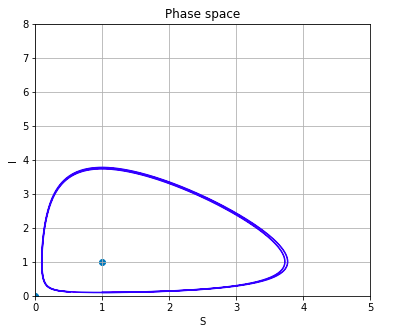
\includegraphics[scale=.5]{images/SI_plane.png}
        
        Figure 1. \textit{Sketch for the S-I plane}
    \end{center}
    
    \begin{flushleft}
        
        The image above was is a closely accurate result to the true plot. However, it is important to note that for different time step, it might affect heavily on the plot that was programmed. As we can see in the following images, especially for those with time step $\Delta = 0.1$ and $\Delta = 0.01$, they are not either not periodic or end up being unstable due to the big gap each time takes.
    \end{flushleft}
    
    \begin{center}
        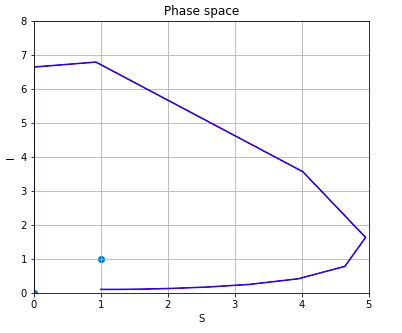
\includegraphics[scale=.5]{images/false_image_1.png}
        
        Figure 2. \textit{Sketch for the S-I plane when $\Delta = 0.1$}
    \end{center}
    
    \begin{center}
        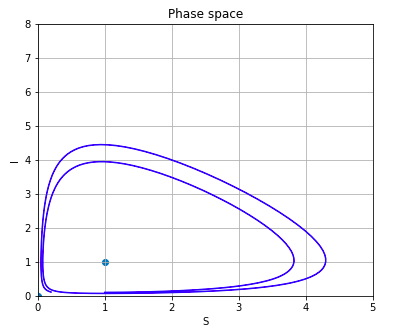
\includegraphics[scale=.5]{images/false_image_2.png}
        
        Figure 3. \textit{Sketch for the S-I plane when $\Delta = 0.01$}
    \end{center}
    
    Other more specific plot can be found in the Jupyter Notebook, that will be attached alongside the document.
\end{document}